\documentclass[a4paper,12pt]{article}
\usepackage[utf8]{inputenc}
\usepackage[french]{babel}
\usepackage[T1]{fontenc}
\usepackage[top=2cm,bottom=2cm,left=2cm,right=2cm]{geometry}
\usepackage{graphicx}
\usepackage{wrapfig}
\usepackage{url}

\begin{document}

\begin{titlepage}
	\begin{center}
		\Large{Année universitaire 2016-2017}\\
		\Large{Université de Caen Normandie}\\[1cm]
		
		\huge{Rapport sur les nouveautés du menu édition}\\
		\vspace{3cm}
		
		Théo Sarrazin
		
	\normalsize{\textit{ ~ L2 Informatique}}\\
		\medskip
		\vspace{2cm}
				
	\end{center}
\end{titlepage}

\tableofcontents
\newpage

\section{Selection de la ligne courante}

	Dans un premier temps, nous avons ajoutés une fonction permettant de selectionner la ligne où ce trouve le curseur.
	Pour cela, nous recuperons l'objet QTextCursor de notre class Editeur (héritant de QTextEdit) puis nous utilisons la méthode \textbf{select} de cet objet qui nous permet de selectionner du texte dans notre Editeur, cette méthode prend en paramètre une méthode de selection, QTextCursor.LineUnderCursor dans notre cas. La ligne ou ce trouve notre cuseur va donc être selectionner.
	Pour appliquer ces modifications, nous devons appliquer notre objet QTextCursor à notre Editeur, pour cela on utilise la méthode \textbf{setTextCursor} de l'objet Editeur et on lui passe en paramètre notre QTextCursor.  


	\begin{figure}[h!]
		\begin{center}
			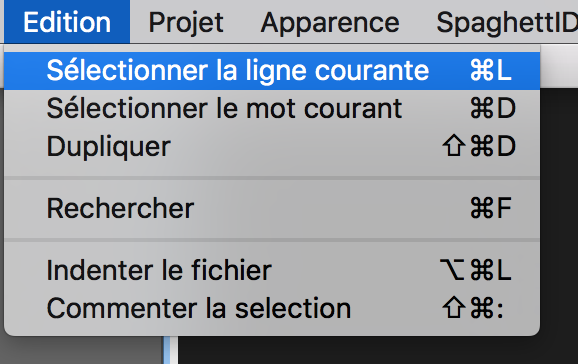
\includegraphics[scale=0.8]{imgs/utilisation_selection_ligne}
			\caption{Action du menu permettant la selection de la ligne courante}
		\end{center}
	\end{figure}

	\begin{figure}[h!]
		\begin{center}
			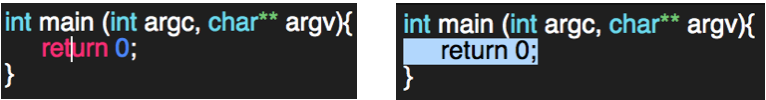
\includegraphics[scale=0.8]{imgs/resultat_selection_ligne}
			\caption{Résultat de l'utilisation de la fonction selection de la ligne courante}
		\end{center}
	\end{figure}

\section{Selection du mot courant}

	Pour l'ajout de la selection du mot courant, la démarche est exactement la même que pour la selection de la ligne courante, nous devons simplement changer la méthode de selection, passant de QTextCursor.LineUnderCursor à QTextCursor.WordUnderCursor, afin de ne plus sélectionner la ligne mais le mot présent au niveau du curseur. 

	\newpage{}

	\begin{figure}[h!]
		\begin{center}
			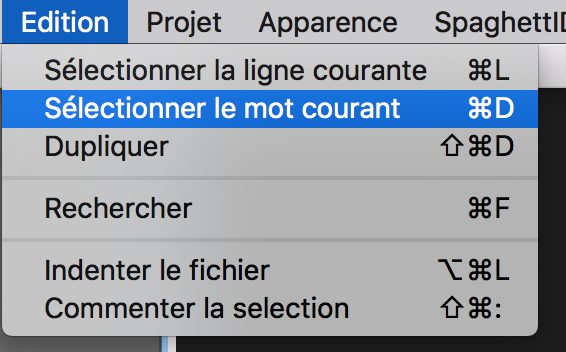
\includegraphics[scale=0.8]{imgs/utilisation_selection_mot}
			\caption{Action du menu permettant la selection du mot courant}
		\end{center}
	\end{figure}

	\begin{figure}[h!]
		\begin{center}
			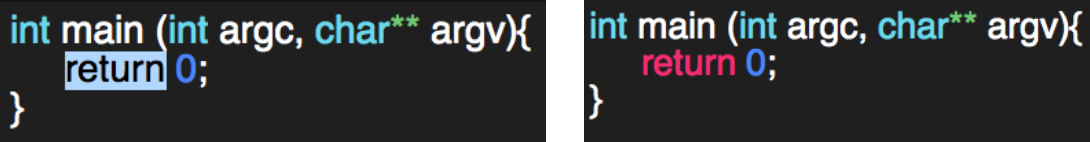
\includegraphics[scale=0.8]{imgs/resultat_selection_mot}
			\caption{Résultat de l'utilisation de la fonction selection du mot courant}
		\end{center}
	\end{figure}

\section{Duplication}

	Pour l'ajout de la duplication du texte, nous avons choisi de différencier deux cas, le premier où rien n'est selectionné et le second où du texte est déjà selectionné. Dans le premier cas toutes la ligne est dupliquée et dans le second seulement la partie selectionnée est dupliquée.

	Pour cela, nous recupperons une nouvelle fois le QTextCursor de notre Editeur, puis pour savoir dans quel cas nous sommes on utilise la méthode selectedText de l'objet QTextCursor. Ainsi si aucun text n'est selectionné nous selectionnons la ligne courante de le même façon que précédement de plus on assigne la valeur  \textbf{\\n} à la variable \textbf{return\_} en effet si on duplique une ligne entière, on ajoute on retoure à la ligne entre la selection d'origine et la partie dupliquée. Puis on ajoute le texte dans notre objet Editeur grâce à la méthode \textbf{inserText} avec en paramètre la selection du QTextCursor (recuperrée grâce à la méthode \textbf{selectedText}) suivi de la variable \textbf{return\_} elle même suivi de la selection du QTextCursor.

	\begin{figure}[h!]
		\begin{center}
			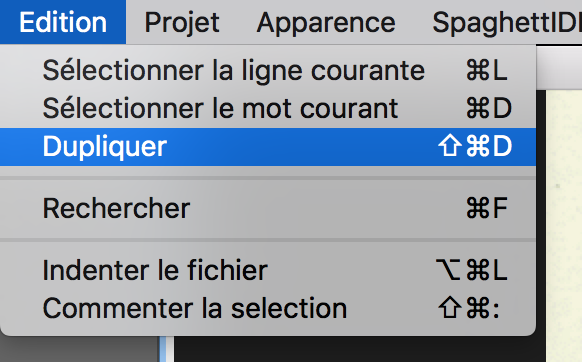
\includegraphics[scale=0.8]{imgs/utilisation_duplication}
			\caption{Action du menu permettant de dupliquer}
		\end{center}
	\end{figure}


	\begin{figure}[h!]
		\begin{center}
			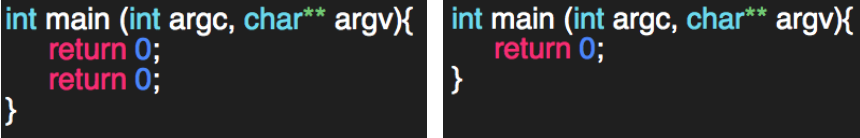
\includegraphics[scale=0.8]{imgs/resultat_duplication}
			\caption{Résultat de l'utilisation de la fonction permettant de dupliquer}
		\end{center}
	\end{figure}

	\newpage{}
\section{Recherche}

	Pour la recherche dans le document, nous avons decidés d'ajouter une boite de dialogue permettant d'entrée le texte à rechercher. Pour cela nous avons créés une classe SearchDialog (héritant de QDialog), lors de l'affichage de cette boite de dialogue nous utilisons la méthode \textbf{exec}, qui rend impossible l'interaction avec la fenetre en arrière plan tant que la boite de dialogue est ouverte.

	Cette boite de dialogue nous permer de taper le texte à rechercher, de choisir si on recherche en avant ou en arrière , mais aussi si on veut être sensible à la case.

	\begin{figure}[h!]
		\begin{center}
			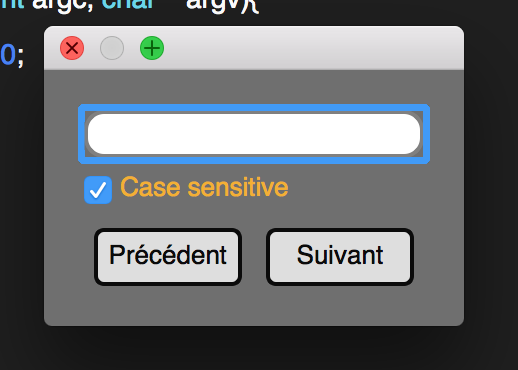
\includegraphics[scale=0.8]{imgs/boite_dialog_recherche}
			\caption{Boite de dialogue relative à la recherche}
		\end{center}
	\end{figure}

	Pour la recherche on utilise la méthode \textbf{find} de notre objet Editeur. Cette méthode prend en paramètre le texte à rechercher, suivit de differents drapeaux. Dans notre cas nous utilisons le drapeau permettant d'executer la rechercher en arrière et le drapeau permettant de faire la recherche en étant sensible à la case (respectivement les drapeaux \textbf{QTextDocument.FindBackward} et \textbf{QTextDocument.FindCaseSensitively})

	\begin{figure}[h!]
		\begin{center}
			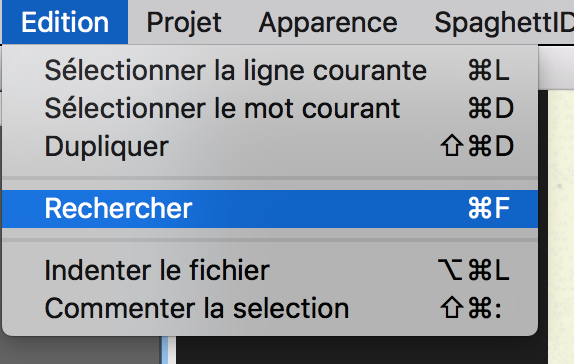
\includegraphics[scale=0.8]{imgs/utilisation_rechercher}
			\caption{Action du menu permettant de dupliquer}
		\end{center}
	\end{figure}

	\begin{figure}[h!]
		\begin{center}
			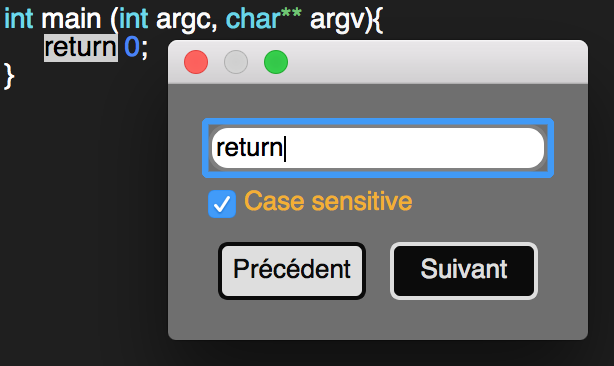
\includegraphics[scale=0.8]{imgs/resultat_rechercher}
			\caption{Résultat de l'utilisation de la fonction permettant de dupliquer}
		\end{center}
	\end{figure}

\section{Indentation du fichier}

	Pour l'indentation du document, nous allons changer son contenue (ajout/retrait de tabulation) nous devons donc stocker la position courante du curseur (grâce à la méthode \textbf{blockNumber} de l'objet QTextCursor). Par la suite on recupère le contenue du document grâce à la méthode \textbf{toPlainText} de l'objet Editeur. On créer une variable \textbf{indent\_level}, qui contient le niveau courant d'indentation, puis on parcoure toutes les lignes de notre document, si le ligne contient le charactère "\}", on retire 1 au niveau d'indentation puis on change la ligne pour ajouter au debut de cette dernière \textbf{indent\_level} fois une tabulation, puis on ajoute 1 au niveau d'indentation si la ligne contient "\{".
	Pour finir on defini le nouveau texte ainsi obtenu comme texte de notre document avec la méthode \textbf{setPlainText} et on replace le curseur au bon endroit.

	\newpage{}

	\begin{figure}[h!]

		\begin{center}
			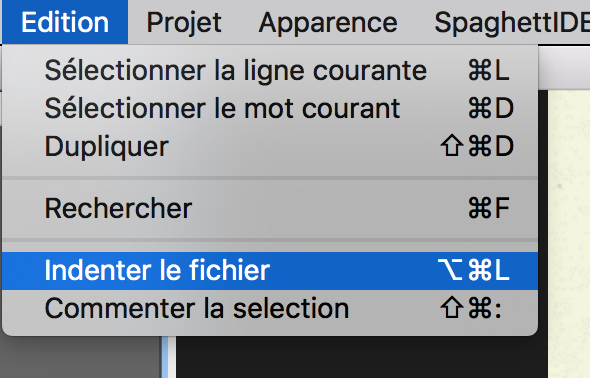
\includegraphics[scale=0.8]{imgs/utilisation_indentation}
			\caption{Action du menu permettant d'indenter le fichier}
		\end{center}
	\end{figure}

	\begin{figure}[h!]
		\begin{center}
			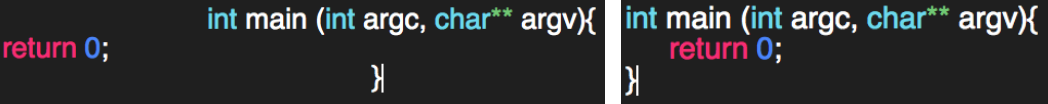
\includegraphics[scale=0.8]{imgs/resultat_indentation}
			\caption{Résultat de l'utilisation de la fonction permettant d'indenter le fichier}
		\end{center}
	\end{figure}

\section{Commenter le fichier}

	De la même façon que pour la duplication du texte, nous avons séparés cette action en deux cas, soit du texte est sélectionné soit rien n'est selectionné.
	Dans le cas ou du text est selectionné nous commenterons seulement à partir du debut de la selection. Si plusieurs lignes sont selectionnées elles seron evidement toutes commentées. Si il n'y a pas de texte selectionné, on commente la ligne courante.

	Dans un premier temps, comme pour la duplication, si rien n'est selectionné on selectionne la ligne courante, puis on sauvegarde le text selectionné que l'on recupère grâce à la méthode \textbf{selectedText}, puis on supprime le texte selectionné avec la méthode \textbf{removeSelectedText}. Pour savoir si le texte est deja commenté, nous parcourons toutes les lignes, si une des lignes ne commence pas par "//" la selection est considérée comme non commenté. Par la suite nous parcourons chaque ligne du texte puis pour chaque ligne nous ajoutons/retirons les charactères "//" en fonction de si le texte et oui ou non déjà commenté.

	Puis on ajoute le texte ainsi modifié à notre document en utilisant la méthode \textbf{insertText} (de l'objet QTextCursor).

	\newpage{}

	\begin{figure}[h!]

		\begin{center}
			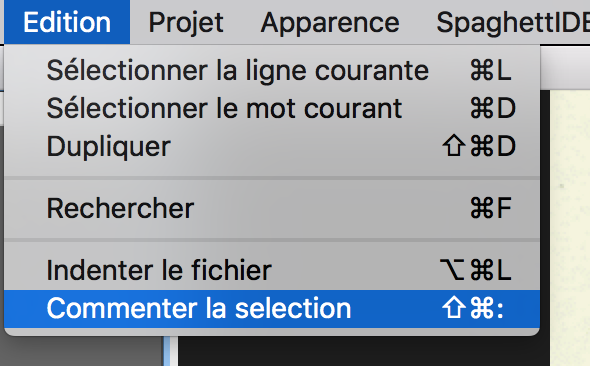
\includegraphics[scale=0.8]{imgs/utilisation_commentaire}
			\caption{Action du menu permettant de commenter le fichier}
		\end{center}
	\end{figure}

	\begin{figure}[h!]
		\begin{center}
			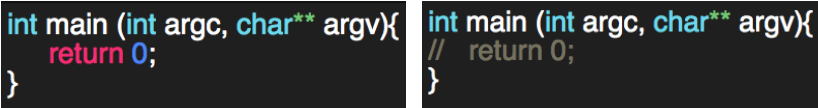
\includegraphics[scale=0.8]{imgs/resultat_commentaire}
			\caption{Résultat de l'utilisation de la fonction permettant de commenter le fichier}
		\end{center}
	\end{figure}

	
\end{document}